%%
%% /docs/poster/poster.tex
%%
%% Created by Paul Warkentin <paul@warkentin.email> on 07/07/2018.
%% Updated by Paul Warkentin <paul@warkentin.email> on 26/07/2018.
%%

\documentclass[a0, portrait]{a0poster}

\usepackage{multicol}
\usepackage[svgnames]{xcolor}
\usepackage{palatino} % \usepackage{times}
\usepackage{graphicx}
\usepackage{booktabs}
\usepackage[font=small,labelfont=bf]{caption}
\usepackage{amsfonts, amsmath, amsthm, amssymb}
\usepackage{wrapfig}
\usepackage{amsmath}
\usepackage{hyperref}

\columnsep=100pt
\columnseprule=2pt
\graphicspath{{figures/}}

\begin{document}

% HEADER

\begin{minipage}[b]{0.75\linewidth}
  \VeryHuge \color{NavyBlue} \textbf{Object Detection with Single Shot MultiBox Detector} \color{Black} \\[3cm]
  \huge \textbf{Paul Warkentin} \\[-0.3cm]
  \Large \texttt{p.warkentin@stud.uni-heidelberg.de} \\[0.5cm]
  \huge University of Heidelberg \\
  \huge Heidelberg Collaboratory for Image Processing (HCI) \\
  \huge Object Recognition and Image Understanding, Prof. Dr. B. Ommer \\%
\end{minipage} %
\begin{minipage}[b]{0.25\linewidth}
  \hspace{-3cm}
  
\includegraphics[height=8cm]{logo_hd.png}
  \hspace{1cm}
  
\includegraphics[height=8cm]{logo_hci.png} \\
\end{minipage}

\vspace{1cm}

\begin{multicols}{3}

% MOTIVATION

\color{Black}

\section*{Motivation}

Reasons why I have chosen this specific project:
\begin{itemize}
  \item Object detection has become more important over the last few years, e.g. in autonomous driving.
  \item By now, there are many different algorithms for object detection published as papers.
  \item Just a few are that lightweight to run them on live inference with an appropriate frame rate.
  \item The Single Shot MultiBox Detector is more efficient on live inference while improving the accuracy at the same time compared to other object detection models like Fast(er) R-CNN and YOLO.
\end{itemize}

% SOLUTION APPROACH

\section*{Single Shot MultiBox Detector}

\subsection*{What does it stand for?}

\begin{itemize}
  \item \textbf{Single Shot:} this means that the tasks of object classification and localization are done in a single forward pass of the network.
  \item \textbf{MultiBox:} this is the name if a technique for bounding box regression developed by \textit{Szegedy et al.}
  \item \textbf{Detector:} the network is an object detector that also classifies those detected objects.
\end{itemize}

\subsection*{Architecture}

\begin{itemize}
  \item The architecture of the SSD model builds on a classifier architecture.
  \item Here the VGG-16 architecture was chosen, but others like ResNet or Inception can also be taken as base network.
  \item The base network is then extended by extra feature layers, thus enabling to extract features at multiple scales and progressively decrease the size of the input to each subsequent layer.
\end{itemize}

\begin{center}\vspace{1cm}
  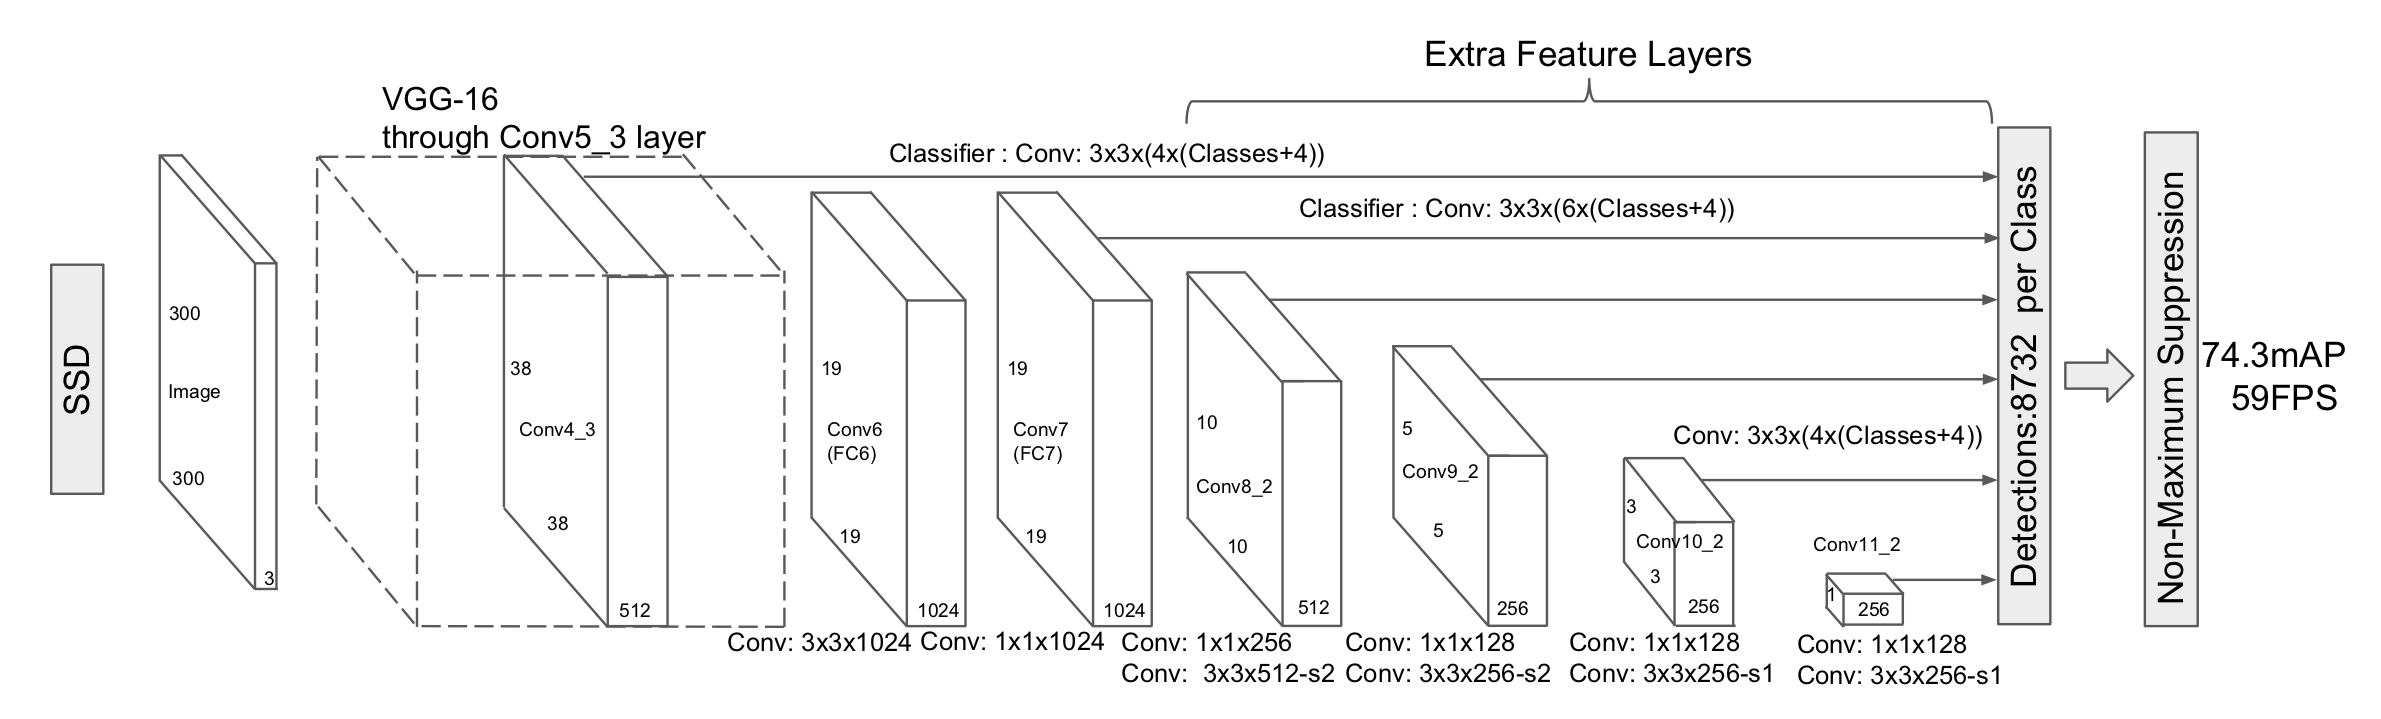
\includegraphics[width=1.0\linewidth]{ssd_architecture.png}
  \captionof{figure}{Architecture of the SSD 300 network.}
\end{center}

\subsection*{MultiBox Priors}

\begin{itemize}
  \item Default anchor boxes are computed for each feature layer for a given set of aspect ratios and scales.
  \item The number of anchor boxes for a feature layer of size $(h, w)$ of $b$ different scales and ratios can be calculated by $b \cdot h \cdot w$.
  \item The SSD 300 in this project has a total of 8732 default anchor boxes.
\end{itemize}

\begin{center}\vspace{1cm}
  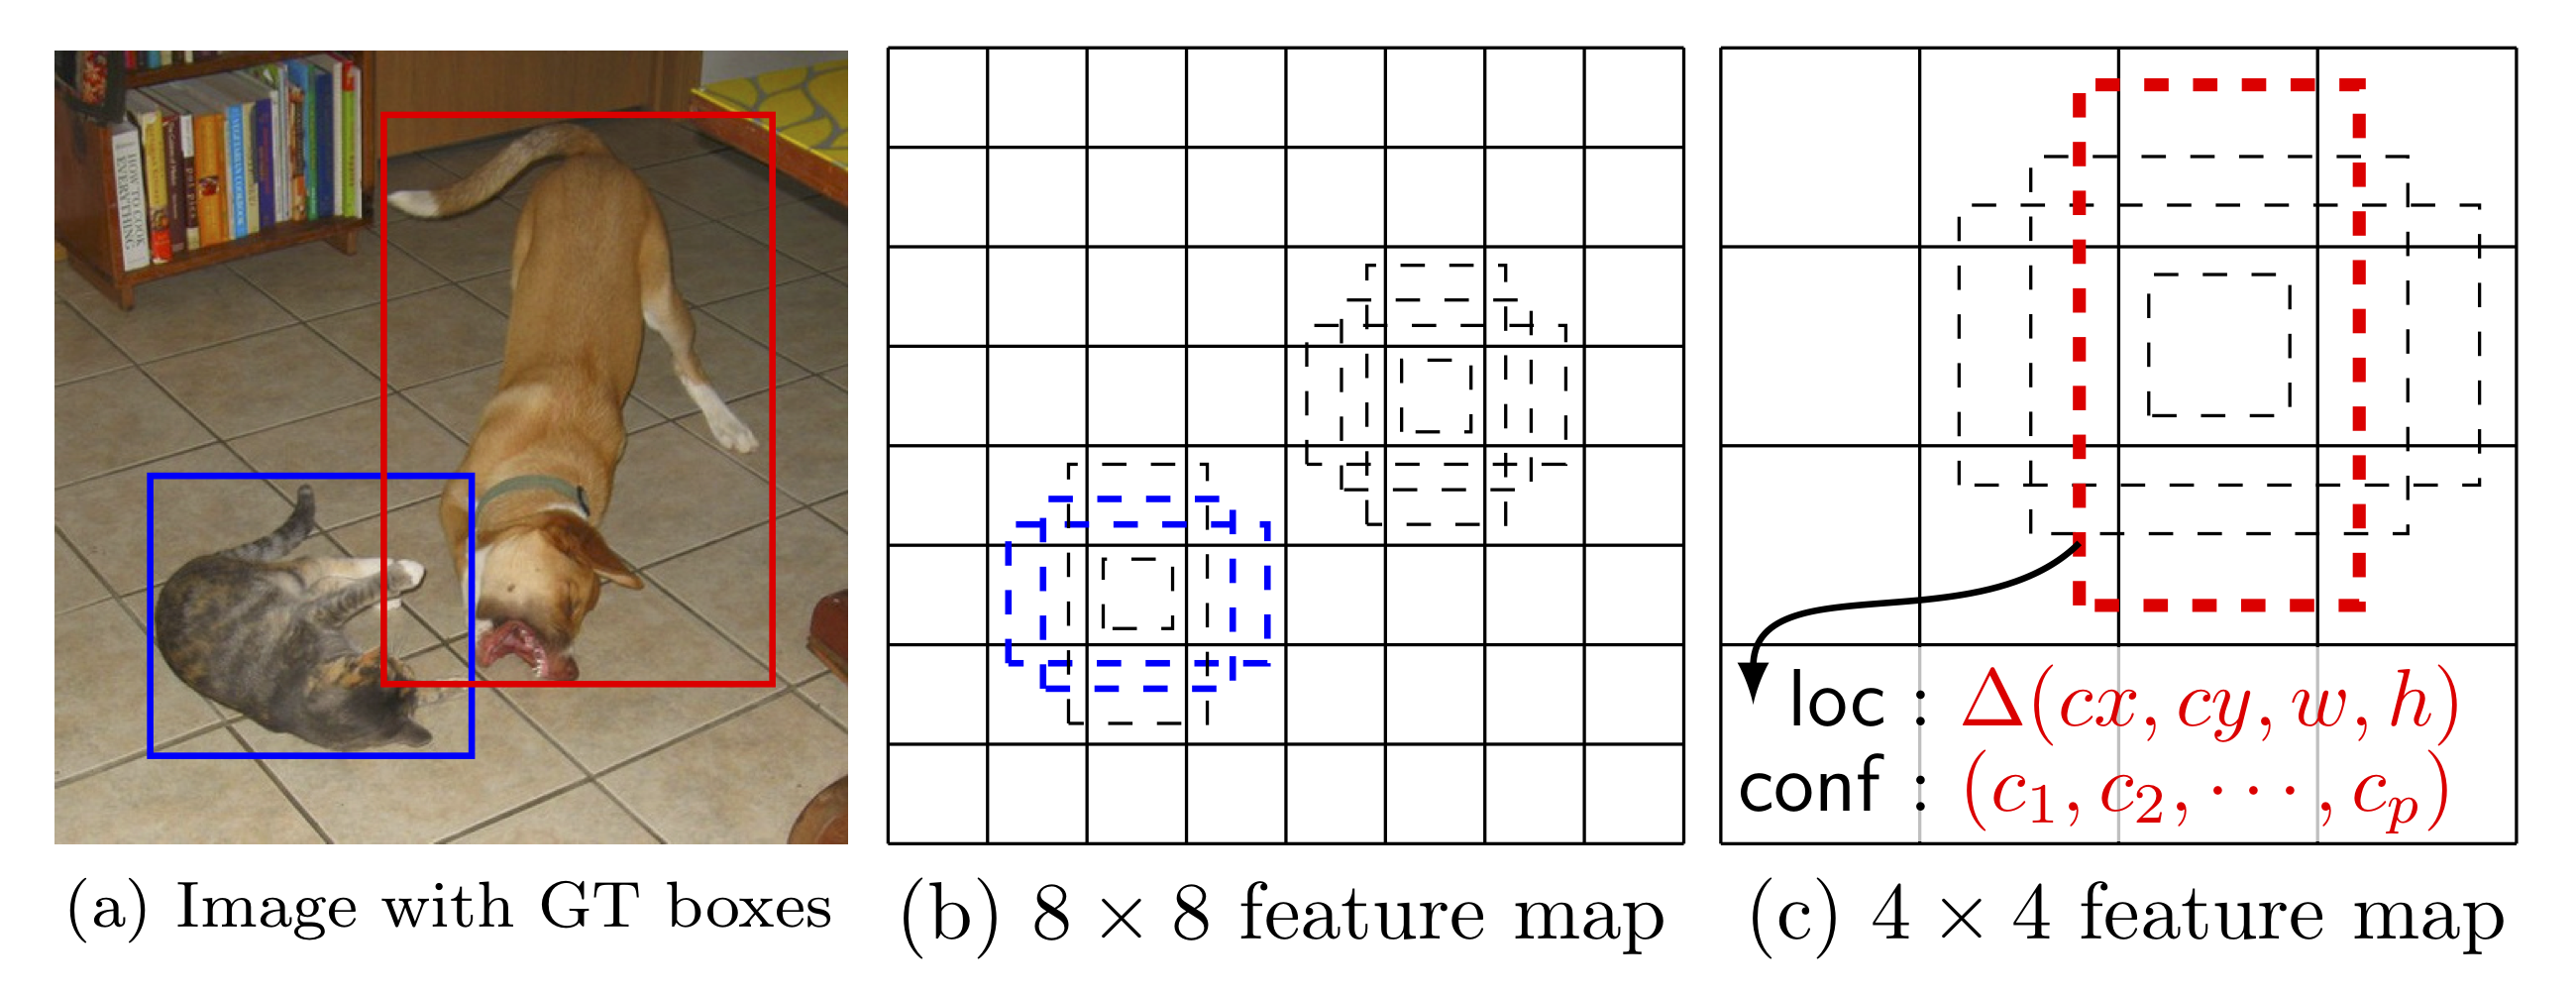
\includegraphics[width=1.0\linewidth]{default_anchor_boxes.png}
  \captionof{figure}{Matching default anchor boxes.}
\end{center}

\subsection*{Loss Function}

\begin{itemize}
  \item Each groundtruth box is matched to the default anchor box with the best Jaccard overlap. Then, default anchor boxes are matched to any groundtruth box with a Jaccard overlap higher than a threshold.
  \item \textbf{Loss:}
  \begin{equation*}
    L(x, c, l, g) = \frac{1}{N}(L_{conf}(x, c) + \alpha L_{loc}(x, l, g)),
  \end{equation*}
  where $x_{ij}^p \in \{0, 1\}$ is an indicator for matching the $i$-th default anchor box to the $j$-th groundtruth box of class $p$.
  \item \textbf{Confidence loss:} For each predicted bounding box, a set of class predictions are computed, for every possible class in the dataset.
  \begin{equation*}
    L_{conf}(x, c) = -\sum_{i \in Pos} x_{ij}^p \log(\hat{c}_i^p) - \sum_{i \in Neg} \log(\hat{c}_i^0),
  \end{equation*}
  for ever groundtruth box $j$, where $\hat{c}_i^p$ is the softmax function over the confidences $c_i^p$.
  \item \textbf{Localization loss:} The localization loss is computed using the smooth L1-Norm.
  \begin{equation*}
    L_{loc}(x, l, g) = \sum_{i \in Pos} \sum_{m \in \{cx, cy, w, h\}} x_{ij}^p \text{smooth}_{L1}(l_i^m - \hat{g}_j^m),
  \end{equation*}
  where $\hat{g}_j^m$ is the SSD encoding of the groundtruth box $j$.
\end{itemize}

\begin{center}\vspace{1cm}
  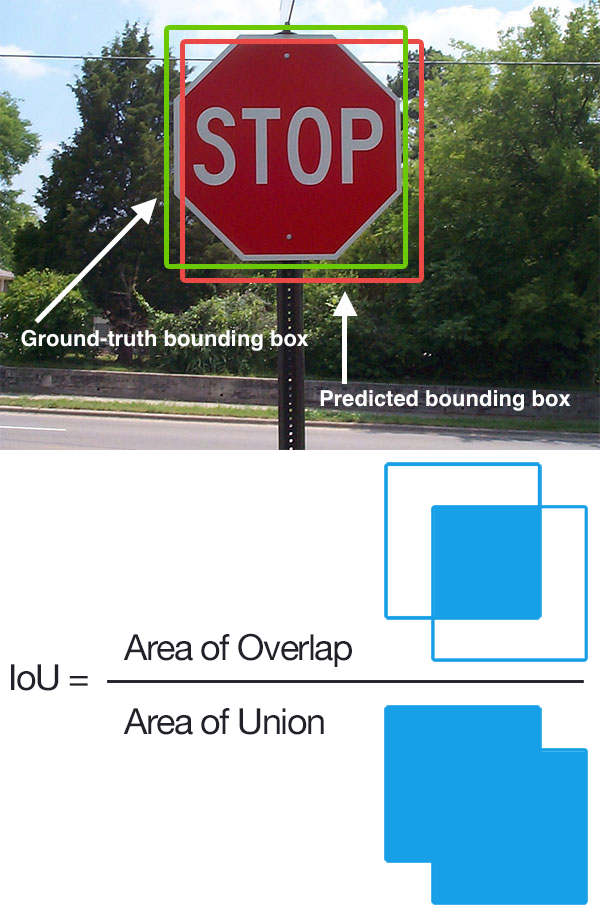
\includegraphics[width=0.6\linewidth]{jaccard_overlap.png}
  \captionof{figure}{Visualization of the Jaccard score / IoU.}
\end{center}

% EVALUATION

\section*{Evaluation}

\begin{itemize}
  \item The metric to evaluate the training results is the mAP (mean average precision).
  \item Consists of the precision and the recall.
  \item \textbf{Precision:} Measures how accurate is the prediction, i.e. the percentage of the positive predictions are correct.
  \item \textbf{Recall:} Measures how good all the positives were found.
\end{itemize}

% RESULTS

\section*{Results}

\subsection*{Training}

\begin{center}\vspace{1cm}
  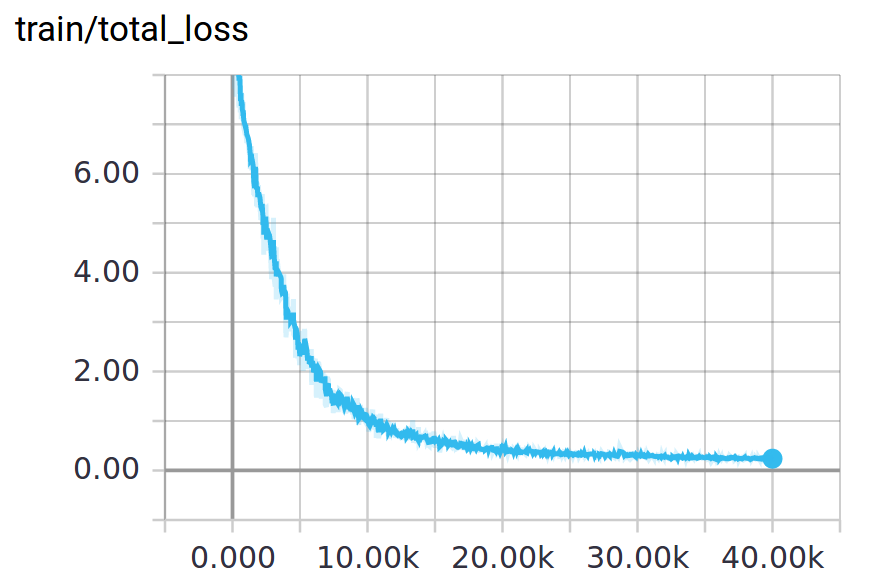
\includegraphics[width=0.45\linewidth]{train_loss_ssd_300.png}
  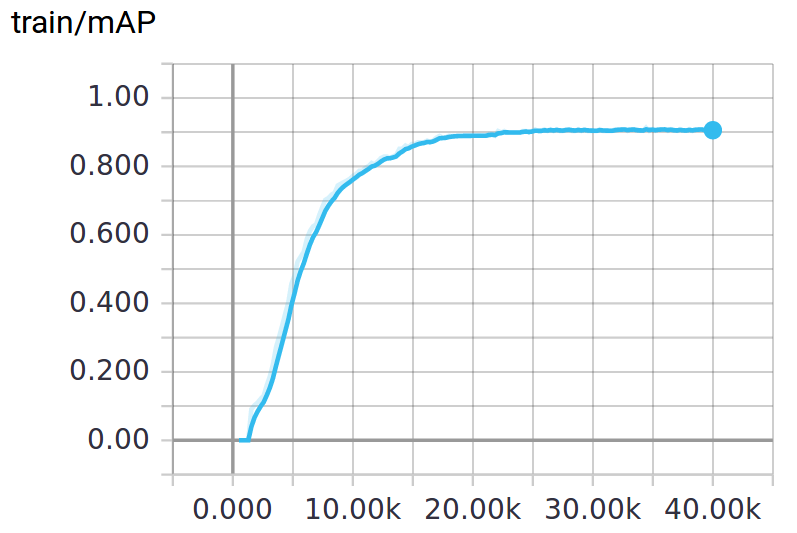
\includegraphics[width=0.45\linewidth]{train_mAP_ssd_300.png}
  \captionof{figure}{Train loss and mAP evolution of SSD 300 network.}
\end{center}

\subsection*{Evaluation}

The following results were evaluated on the Pascal VOC 2007 test set.
\begin{center}\vspace{1cm}
  \begin{tabular}{rl|c|r}
    & \textbf{Method} & \textbf{Dataset} & \textbf{mAP} \\ \cline{2-4}
    & Fast R-CNN & VOC 2007+2012 & 70.00\% \\
    & Faster R-CNN & VOC 2007+2012 & 76.80\% \\ \cline{2-4}
    & SSD 300 & VOC 2007+2012 & 74.30\% \\
    & SSD 512 & VOC 2007+2012 & 76.80\% \\ \cmidrule(r){2-4} \morecmidrules \cmidrule(r){2-4}
    $\times$ & SSD 300 & VOC 2007+2012 & 49.09\% \\
    $\times$ & SSD 512 & VOC 2007+2012 & 54.37\%
  \end{tabular}
  \captionof{table}{Results compared to the paper.}
\end{center}

\subsection*{Inference time}

The paper used a Titan X and cuDNN 4 with Intel Xeon E5-2667v3 @ 3.20GHz. The results of this project were tested using a GTX 1080 Ti and cuDNN 9.0 with Intel Core i7-6850K.
\begin{center}\vspace{1cm}
  \begin{tabular}{rl|c|c|c|c|c}
    & \textbf{Method} & \textbf{mAP} & \textbf{FPS} & \textbf{BS} & \textbf{\# Boxes} & \textbf{Resolution} \\ \cline{2-7}
    & Faster R-CNN & 73.2\% & 7 & 1 & $\sim$ 6000 & $\sim$ 1000 $\times$ 600 \\ \cline{2-7}
    & Fast YOLO & 52.7\% & 155 & 1 & 98 & 448 $\times$ 448 \\
    & YOLO & 66.4\% & 21 & 1 & 98 & 448 $\times$ 448 \\ \cline{2-7}
    & SSD 300 & 74.3\% & 46 & 1 & 8732 & 300 $\times$ 300 \\
    & SSD 512 & 76.8\% & 19 & 1 & 24564 & 512 $\times$ 512 \\
    & SSD 300 & 74.3\% & 59 & 8 & 8732 & 300 $\times$ 300 \\
    & SSD 512 & 76.8\% & 22 & 8 & 24564 & 512 $\times$ 512 \\ \cmidrule(r){2-7} \morecmidrules \cmidrule(r){2-7}
    $\times$ & SSD 300 & 49.09\% & 49 & 1 & 8732 & 300 $\times$ 300 \\
    $\times$ & SSD 512 & 54.37\% & 35 & 1 & 24564 & 512 $\times$ 512
  \end{tabular}
  \captionof{table}{Results compared to the paper.}
\end{center}

\subsection*{Differences to the paper}

\begin{itemize}
  \item Slightly different data augmentation as in the paper.
  \item Slightly different pre- and post-processing as in the paper.
  \item The implementation of the paper was written in Caffe, this projects' implementation was written in TensorFlow.
\end{itemize}

% SAMPLE IMAGES

\section*{Sample images}

In the samples below, one can see that the model works very good on some images, but often the localization and even the classification of objects is not right. One drawback of the SSD model implemented in this project is that it is not good in detecting small objects. By playing around with the hyperparameters and enough training data, this can be improved.
\begin{center}\vspace{1cm}
  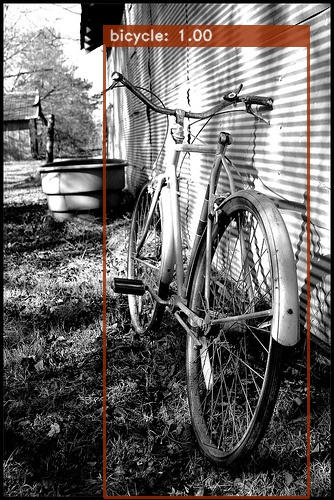
\includegraphics[width=0.3\linewidth]{sample_0_0.jpg}
  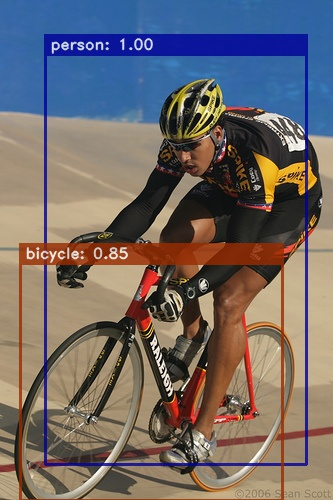
\includegraphics[width=0.3\linewidth]{sample_0_1.jpg}
  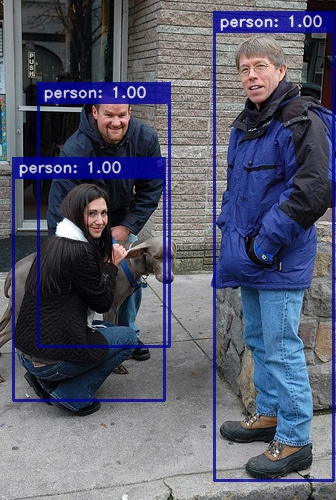
\includegraphics[width=0.3\linewidth]{sample_0_2.jpg}
  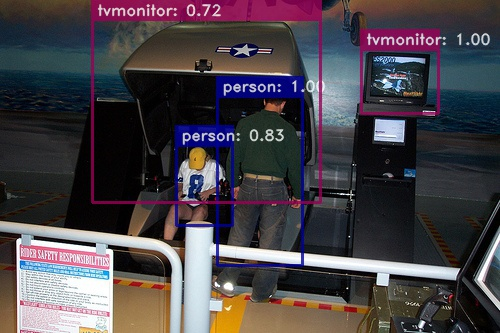
\includegraphics[width=0.3\linewidth]{sample_1_0.jpg}
  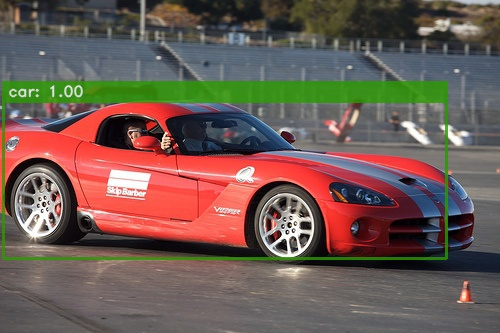
\includegraphics[width=0.3\linewidth]{sample_1_1.jpg}
  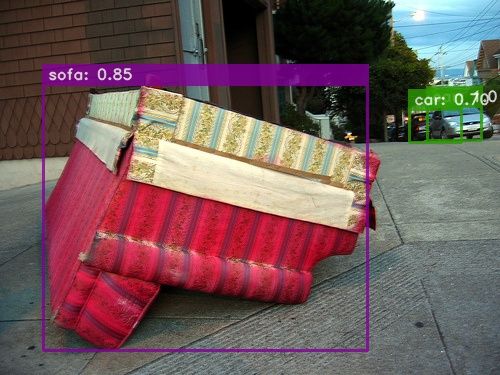
\includegraphics[width=0.3\linewidth]{sample_1_2.jpg}
  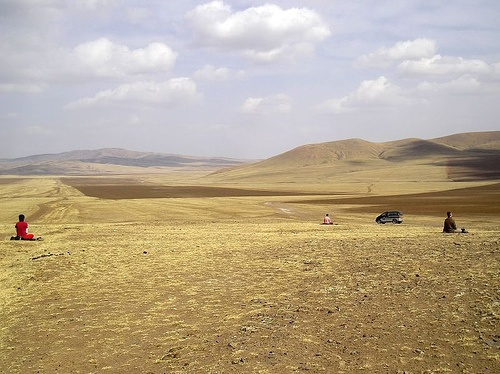
\includegraphics[width=0.3\linewidth]{sample_2_0.jpg}
  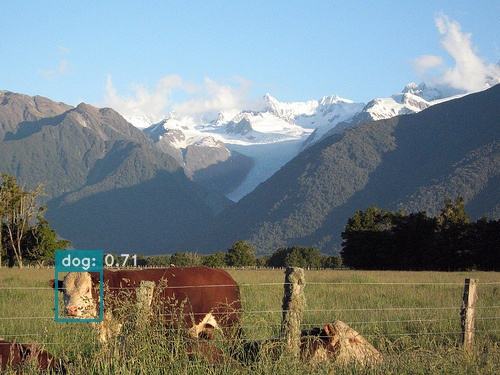
\includegraphics[width=0.3\linewidth]{sample_2_1.jpg}
  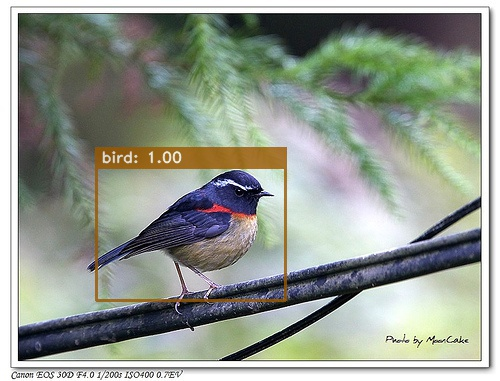
\includegraphics[width=0.3\linewidth]{sample_2_2.jpg}
  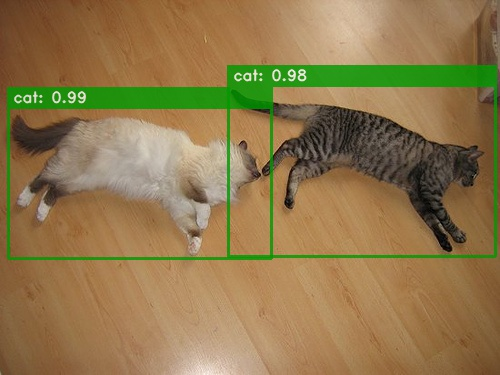
\includegraphics[width=0.3\linewidth]{sample_3_0.jpg}
  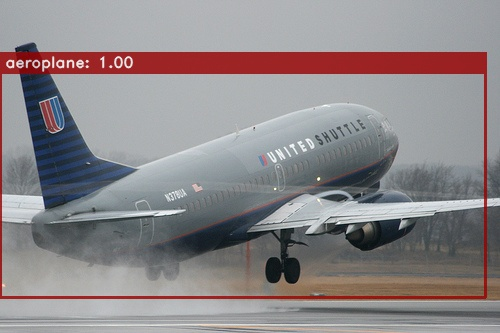
\includegraphics[width=0.3\linewidth]{sample_3_1.jpg}
  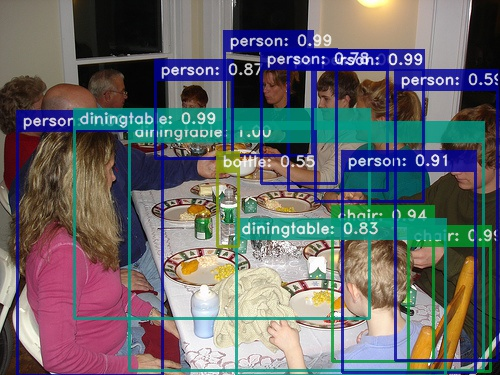
\includegraphics[width=0.3\linewidth]{sample_3_2.jpg}
  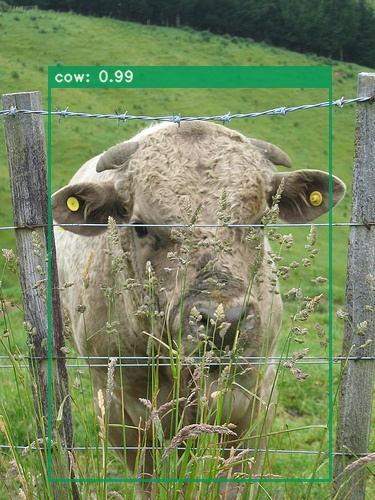
\includegraphics[width=0.3\linewidth]{sample_4_0.jpg}
  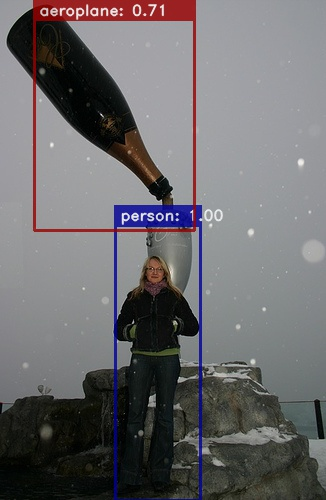
\includegraphics[width=0.3\linewidth]{sample_4_1.jpg}
  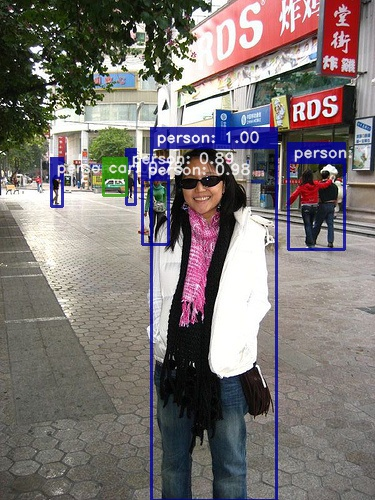
\includegraphics[width=0.3\linewidth]{sample_4_2.jpg}
  \captionof{figure}{Sample annotated with SSD 300.}
\end{center}

% RESOURCES

\section*{Resources}

\begin{itemize}
  \item Original paper about SSD: \\
  https://arxiv.org/pdf/1512.02325.pdf
\end{itemize}

\end{multicols}
\end{document}
